%%%%
%       _  _____  ___  _____  _   _  ___ 
%      / \|_   _||_ _||_   _|| | | |/ __|
%     / △ \ | |   | |   | |  | |_| |\__ \
%    /_/¯\_\|_|  |___|  |_|   \___/ |___/
%                 EDUCAÇÃO
%    Modelo de TCC - Ciência da Computação
%%%%

\documentclass[12pt]{article}
\usepackage{physics}
\usepackage{sbc-template}
\usepackage{graphicx, url}
\usepackage[utf8x]{inputenc}
\usepackage[brazil]{babel}
\usepackage[T1]{fontenc}
\usepackage[english=american]{csquotes}
\usepackage{float}
\usepackage{comment}
\usepackage{amsmath}
\usepackage{amssymb}
\usepackage{enumerate}
\usepackage{subcaption}
\usepackage{setspace}
\usepackage{listings}
\usepackage{inconsolata}
\usepackage{tabularray}
% acrescimos
\usepackage{xcolor}
\usepackage{multicol}

%\usepackage[backref=page]{hyperref}
%\hypersetup{
%    colorlinks=true,
%    allcolors=blue,
%}

% %%%%%%%%%%%%%%%%%%%%%%%%%%%%%%%%%%%%%%%%%%%%%%%%%%%%%%%%%%%%%%
% define o modelo de referencias
\usepackage[style=abnt]{biblatex}

% indica o arquivo com as referencis bibliograficas
\addbibresource{sbc-template.bib}

% carrega o pacote com alterações para Computação Atitus
\usepackage{sty/cc_atitus}
% %%%%%%%%%%%%%%%%%%%%%%%%%%%%%%%%%%%%%%%%%%%%%%%%%%%%%%%%%%%%%%

% %%%%%%%%%%%%%%%%%%%%%%%%%%%%%%%%%%%%%%%%%%%%%%%%%%%%%%%%%%%%%%
% REFERENCIAS DEVERÃO SER INCLUÍDAS NO ARQUIVO: sbc-template.bib
%
% SOBRE CITAÇÕES:
% Para citar no padrão '(Autores, ano)' use: \cite{chave}
% Para citar no padrão 'Autores (ano)'  use: \textcite{chave} ou \citeonline{chave}
% Para citar no padrão 'Autores'        use: \citelastname{chave}
% Para citar no padrão '(Autor, 2009c; Outro Autor, 2009; Outro Autor, 2015)' use: \cites{chave1}{chave2}{chave3}
% Para citar no padrão 'Autor (ano), Autor (ano) e Autor (ano)' use: \textcites{chave1}{chave2}{chave3}

% Demais exemplos ver documento:
%  https://github.com/abntex/biblatex-abnt/raw/master/doc/biblatex-abnt.pdf
%
% Normas ABNT: https://usp.br/sddarquivos/arquivos/citacoes10520.pdf
%              https://usp.br/sddarquivos/arquivos/abnt6023.pdf
%
% %%%%%%%%%%%%%%%%%%%%%%%%%%%%%%%%%%%%%%%%%%%%%%%%%%%%%%%%%%%%%%
% Atualizações no modelo
% 2024-09-23: (fahadkalil) Ajuste para quebra automática de linhas nas células de uma tabela
% 2024-10-17: (fahadkalil) Inserção de comentários com outras citações e indicação de uso do comando "\enquote"
% %%%%%%%%%%%%%%%%%%%%%%%%%%%%%%%%%%%%%%%%%%%%%%%%%%%%%%%%%%%%%%
% CABEÇALHO
\title{Manual Prático do Executor} % titulo

\author{Nome aluno\inst{1}, Nome orientador\inst{1}} % autor principal, orientador

\address{Ciência da Computação -- Atitus Educação\\
Passo Fundo -- RS -- Brasil
\email{aluno@atitus.edu.br, orientador@atitus.edu.br}
}
% %%%%%%%%%%%%%%%%%%%%%%%%%%%%%%%%%%%%%%%%%%%%%%%%%%%%%%%%%%%%%%

\begin{document}
\maketitle % Não remova essa linha!

\begin{abstract} % resumo em inglês
  Escreva seu resumo em língua estrangeira (inglês)...
\end{abstract}
     
\begin{resumo}
  Resumo do trabalho (português)...  
\end{resumo}
\fontfamily{qag}\selectfont
\section{Cabos Sintenax Antiflam Unipolares }

\begin{minipage}[t]{\linewidth}\color{blue}
	\centering
	\noindent
	\texttt{NBR 7288}
\end{minipage}
\rule{\linewidth}{.1em}\par
\noindent
\begin{tabular}{|c|c|c|}
	\hline
	Bitola & Capacidade de  & Seção Nominal \\
	 & Condução de Corrente & \\
	(AWG / MCM) & (A) & $(mm^{2})$ \\
	\hline
	14 & 15,5 & 1,5 \\
	\hline
	12 & 21,0 & 2,5 \\
	\hline
	10 & 28,0 & 4 \\
	\hline
	8 & 36,0 & 6 \\
	\hline
	6 & 50,0 & 10 \\
	\hline
	4 & 68,0 & 16 \\
	\hline
	2 & 89,0 & 25 \\
	\hline
	1 & 111,0 & 35 \\
	\hline
	1/0 & 134 & 50 \\
	\hline
	2/0 & 171 & 50 \\
	\hline
	3/0 & 171 & 70 \\
	\hline
	4/0 & 207 & 95 \\
	\hline
	250 & 239 & 120 \\
	\hline
	300 & 239 & 120 \\
	\hline
	350 & 272 & 150 \\
	\hline
	400 & 310 & 185 \\
	\hline
	500 & 364 & 240 \\
	\hline
	& 419 & 300 \\
	\hline
	& 502 & 400 \\
	\hline
	& 578 & 500 \\
	\hline
\end{tabular}
\section{Fórmulas Práticas}
Circuitos CC\\
Lei de Ohm
\begin{multicols}{3}
$U\, =\, R\, I$ \par
$I\, =\, \frac{U}{R}$ \par
$R\, =\, \frac{U}{I}$
\end{multicols}
Potência
\begin{multicols}{3}
$P\, =\, U\, I$ \par
$P\, =\, I^2\, R$ \par
$R\, =\, \frac{U^2}{R}$
\end{multicols}
\begin{description}
    \item[U] - Tensão (volts)
    \item[I] - Corrente (ampéres)
    \item[R] - Resistência (ohms)
    \item[P] - Potência (watts)
\end{description}
\begin{comment}
testando comentario
\end{comment}

Circuitos CA \\
Impedências Reatâncias \par
$Z\,=\, \sqrt{R^2 + \qty(X_\mathrm{L} - X_\mathrm{C})^2}$


\begin{description}
    \item[Exemplos de citação indireta]    
\end{description}

Segundo \textcite{spinello2024}, o trabalho de conclusão deve ter citações retiradas de artigos científicos encontrados nas bases de dados. 

O trabalho de conclusão deve ter citações retiradas de artigos científicos encontrados nas bases de dados \cite{spinello2024}.

\begin{description}
    \item[Exemplos de citação direta curta]
\end{description}

Segundo \textcite{spinello2024} \enquote{o trabalho de conclusão deve ter citações retiradas de artigos científicos encontrados nas bases de dados}. Note que para colocar um texto entre aspas, usamos o comando \verb|\enquote{texto}|.

Ressalta-se que o \enquote{trabalho de conclusão deve ter citações retiradas de artigos científicos encontrados nas bases de dados} \cite{spinello2024}.

No estudo comparativo apresentado em \textcite[p. 107]{rabello2010} ...

No trabalho de \textcite{pargaonkar2021} ...

No artigo de \textcite{estevao2023} ...

\textsc{Citação direta longa devem ser evitadas em artigos científicos!}

\section{Trabalhos Relacionados}

Trabalhos semelhantes aos objetivos específicos, sempre detalhando ao final da seção a
diferença ao trabalho proposto (quantidade -- 5 trabalhos);

Neste item serão apresentados os principais trabalhos que possuem uma relação com o assunto definido neste estudo....

% Itens com marcadores
\begin{itemize}
     \item \textbf{Título do artigo 01 \cite{ogliari2019}}
     
     Primeiro parágrafo indicar uma introdução do assunto... \\
     No segundo: o que o estudo procurou analisar, qual o objetivo... \\
     No terceiro: o que foi desenvolvido, qual aplicação/experimento foi realizado... \\
     Último: em quais conclusões o trabalho chegou... \\
         
    \item \textbf{Título do artigo 02 (Autor, ano)}
    
     Primeiro parágrafo indicar uma introdução do assunto... \\
     No segundo: o que o estudo procurou analisar, qual o objetivo... \\
     No terceiro: o que foi desenvolvido, qual aplicação/experimento foi realizado... \\
     Último: em quais conclusões o trabalho chegou... \\
    
    \item \ldots
\end{itemize}

\section{Materiais e Métodos}
    Tecnologias, instrumentos e procedimentos que serão usados no estudo. O Algoritmo \ref{alg:id_algo} se refere ao método de ordenação Bubblesort expresso em linguagem Python.

    % Código-fonte formatado
    % Ver: https://en.wikibooks.org/wiki/LaTeX/Source_Code_Listings
    \begin{lstlisting}[  
        %float,
        language=Python, 
        frame=single, 
        numbers=left,
        caption={Método de ordenação Bubblesort},
        label={alg:id_algo} % id para referenciar
        ]        
    def bubble_sort(alist):
        for i in range(len(alist)-1,0,-1):
            for j in range(i):
                if alist[i]>alist[i+1]:
                    temp = alist[i]
                    alist[i] = alist[i+1]
                    alist[i+1] = temp    
    \end{lstlisting}

    % Figura
    % https://pt.overleaf.com/learn/latex/Inserting_Images
    \begin{figure}[H]
        \centering
        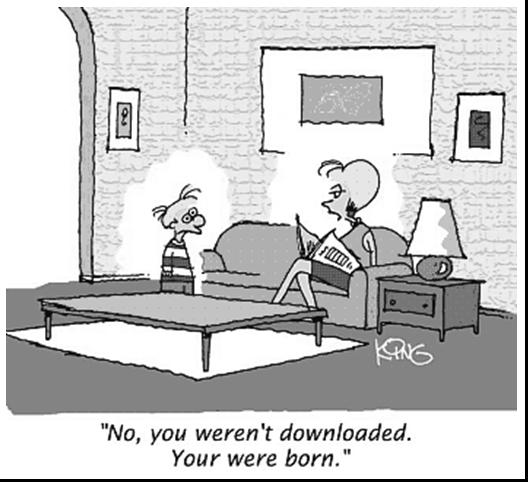
\includegraphics[width=0.5\textwidth]{fig1.jpg}
        \caption{Minha figura}
        \label{fig:id_figura}
    \end{figure}
    
    % Tabela
    % Editor online: https://www.latex-tables.com
     \begin{table}[ht]
        \centering
        \caption{Minha tabela}
        \label{tab:id_tabela}
        \begin{tblr}{
          colspec = {X[l] X[l]}, % Tipo X define células com quebra automática de linha. Use: l=left, r=right, c=center ou j=justify para alinhamento dentro das células
          width = \linewidth,
          hlines, % inclui borda horizontal
          vlines, % inclui borda vertical        
        }
        \textbf{cabeçalho 1} & \textbf{cabeçalho 2} \\
        {texto à esquerda} & {Existem muitas variações das passagens do Lorem Ipsum disponíveis, mas a maior parte sofreu alterações de alguma forma, pela injecção de humor, ou de palavras aleatórias que nem sequer parecem suficientemente credíveis. Se vai usar uma passagem do Lorem Ipsum, deve ter a certeza que não contém nada de embaraçoso escondido no meio do texto.}
        \end{tblr}
    \end{table}

\section{Resultados e Discussão}
Essa seção deverá ser escrita na segunda parte do trabalho, conhecida como TCC2.

\section{Considerações Finais}
Essa seção deverá ser escrita na segunda parte do trabalho, conhecida como TCC2.

% %%%%%%%%%%%%%%%%%%%%%%%%%%%%%%%%%%%%%%%%%%%%%%%%%%%%%%%%%%%%%%
% Seção de Referências (gerada automaticamente)
\printbibliography  % Não remover esta linha
% %%%%%%%%%%%%%%%%%%%%%%%%%%%%%%%%%%%%%%%%%%%%%%%%%%%%%%%%%%%%%%

\end{document}